\section{GRU}
LSTM'e benzerdir. Daha az tensör işlemine sahiptir bu yüzden LSTM'den daha hızlı çalışır. LSTM'den farklı olarak bilgi aktarmak için gizli katmanları kullanır. İki kapıdan oluşur.

\begin{itemize}
    \item \textbf{Update Gate:} Bilgilerin unutulup unutulmayacağına karar verir.
    \item \textbf{Reset Gate:} Ne kadar bilginin unutulacağına karar verir.
\end{itemize}

\begin{figure}[h]
    \centering
    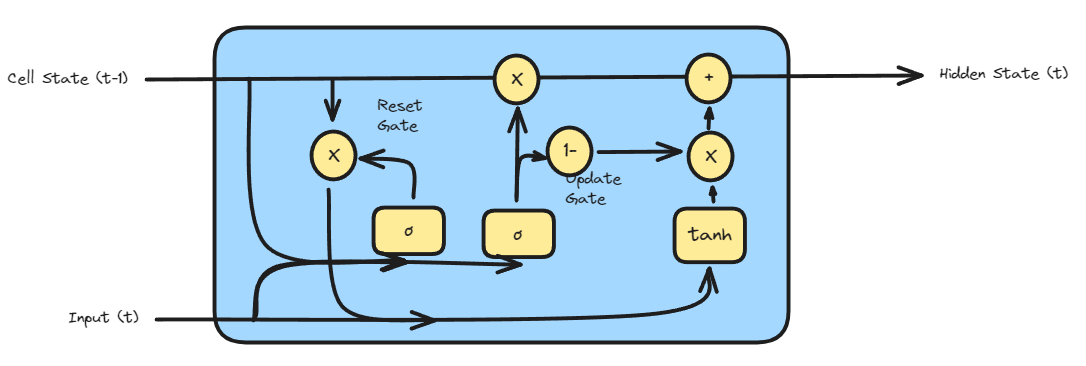
\includegraphics[width=1\textwidth]{images/gru_layer.png}
    \caption{GRU katmanı.}
    \label{fig:enter-label}
\end{figure}

\newpage